% Doc Setup
\documentclass[11pt]{article}
\usepackage{setspace} 
\doublespacing
\usepackage{amsmath}
\usepackage{graphicx} % Required for inserting images
\usepackage{titlesec} % For custom section titles
\usepackage{lipsum}
\usepackage{hyperref}
\usepackage{float}
\usepackage{mathptmx} % Times New Roman
\usepackage{booktabs}
\usepackage{subcaption}


\usepackage[letterpaper,top=1in,bottom=1in,left=1in,right=1in,marginparwidth=1.75cm]{geometry}


\title{STA 137 Final Project}
\author{Ryan Chiang, Manik Sethi, Muhammad Laiq, Tyler Le, Talha Shafik}
\date{June 2025}
\usepackage{listings}
\begin{document}

\maketitle


\begin{figure}[H]
    \centering
    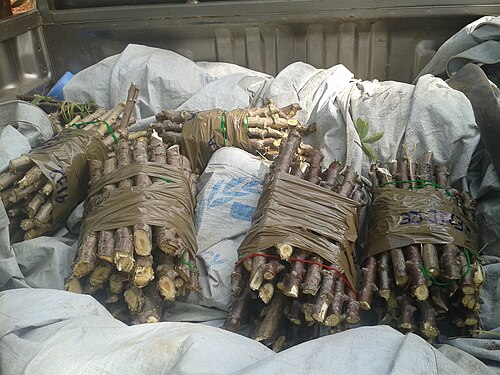
\includegraphics[width=0.3\linewidth]{central_africa_republic.jpg}
    \caption{Central African Lumber}
    \label{fig:enter-label}
\end{figure}




\tableofcontents

%Command for sectioning parts
\newcommand{\numberedpart}[1]{%
    \part{#1}%
}

\section{Introduction}

Agriculture is a vital part of the Central Africa Republic's (CAR) economy, occupying nearly four-fifths of the national work force (Ref 1). Goods such as crops, timber and diamonds are essential, and the hallmark of CAR's economy. However, it is rare that these goods stay within the republic itself. Many of these items make their way out of the country as exports, which in turn provide capital to keep the country running.
Studying the trends of GDP and Exports over time allows us to be informed when deciding whether or not the Central African Republic should agree to certain trade deals. By knowing how dependent CAR is on the wealth of other countries, a delicate balance between domestic independence and international exploitation can be found. Time series analysis will offer insights into year-long trends of the economy.


\section{Explanatory Data Analysis}

For our explanatory data analysis, we will start by looking at our GDP Data. Plotting our data with 'year' on the x-axis (Fig. 2a), we are able to eye-ball the general trend and seasonality. There seem to be two bumps, each separated by approximately twenty years. To verify that this "seasonality" really does exist, we plot the moving average with a lag of 5 and see the two bumps still exist (Fig. 2c). To check if our GDP has a stable variance overtime, we calculate the standard deviation over five years and overlay the graph on top of our regular time series (Fig. 2e). This plot reveals to us that our standard deviation hovers around \$150 million, but quickly jumps up to values of \$250 million during periods of intense growth or recession.

Moving on to our Imports Data, we start off by creating a simple time series of Imports (in millions) by time. (Fig. 2b). It's difficult to discern a trend, as the number of imports goes down from 1960 to 2000, but then starts to rebound up. Whether this is a part of a season whose cycle is longer that the years recorded is unclear, and will require some research into current CAR economic policies to say for sure. What is clear though, is the volatility of our data (Fig. 2f). Compared to our GDP data, the imports seem a lot more noisy.

Looking at these plots reveal the presence or absence of trends and seasonality in GDP and Imports data. Using this, we are able to make informed decisions on transformations needed to make our data meet the assumptions used for commonly-used time series models.



\section{Model Selection}

\subsection{Transformation}
  \subsubsection{GDP}
   The raw GDP time series exhibits a clear upward trend over time, suggesting non-stationarity. This is important because ARIMA models assume constant mean and variance over time. We transform the data, to prevent any model misfit which may produce misleading inferences and poor forecasts. To stabilize the variance and better interpret changes over time, we applied a log transformation to the GDP values:
\[Y_t = \log(\text{GDP}_t)\]   

After transforming the data, we applied first differencing to remove the non-stationary trend component. The resulting series \( Z_t \) appears to fluctuate around a constant mean and shows more stable variance, indicating that it may now be stationary.


\begin{figure}[H]
  \centering
  \includegraphics[width=0.6\linewidth]{transformation.JPEG}
  \caption{Transformation of GDP series} 
  \label{fig:transformation}
\end{figure}

  \subsubsection{Import Model}
  % …your notes on transforming the imports series…

\subsection{ACF/PACF}
To determine potential models for ARIMA, we examine the ACF and PACF of the transformed series.

\begin{itemize}
    \item \textbf{ACF:} The ACF plot of the differenced series shows a spike at lag 1, then followed by a gradual decay. This behavior is similar to a Moving Average (MA) process.

    \item \textbf{PACF:} The PACF does not show a show a strong cut-off pattern, with nshowing ashowing a strong significance beyond the noise band. This suggests a lack of strong Autoregressive (AR) behavior, indicating the AR component might not be necessary.
\end{itemize}


\begin{figure}[h]
  \centering
  \includegraphics[width=1.0\linewidth]{ACF.JPEG}
  %\caption{ACF Plot of Differenced log(GDP)}
  %\label{fig:acf}
\end{figure}

  \subsubsection{GDP}
  
  % …ACF/PACF plots and discussion for GDP…
  \subsubsection{Import Model}
  % …ACF/PACF plots and discussion for imports…

\subsection{Candidate Models}
  \subsubsection{GDP}
Our Candidate Models were MA(1), MA(2), ARMA(1,1), and ARIMA(0,1,1). Evaluating the AIC, AICc, and BIC of each of the models returned the following results:
\begin{figure}
    \centering
    \includegraphics[width=1\linewidth]{CandidateTable.png}
    \caption{Comparison Statistics}
    \label{fig:aic}
\end{figure}
As outlined in Figure 3, the model with the lowest AIC, AICc, and BIC is ARMA(1,1). This is a good indicator that our final model for GDP should be ARMA(1,1). However, we will look at residual plots to double check and look for trends in our QQ-plot that might indicate non-normal residuals. 

\begin{document}

\begin{figure}[ht]
  \centering
  % First row of residuals
  \begin{subfigure}[b]{0.45\textwidth}
    \includegraphics[width=\textwidth]{MA1residuals.png}
    \caption{MA(1) Residuals}
    \label{fig:MA1res}
  \end{subfigure}%
  \hfill
  \begin{subfigure}[b]{0.45\textwidth}
    \includegraphics[width=\textwidth]{MA2residuals.png}
    \caption{MA(2) Residuals}
    \label{fig:MA2res}
  \end{subfigure}

  \vspace{0.5\baselineskip}

  % Second row of residuals
  \begin{subfigure}[b]{0.45\textwidth}
    \includegraphics[width=\textwidth]{ARMAresiduals.png}
    \caption{ARMA(1,1) Residuals}
    \label{fig:ARMAres}
  \end{subfigure}%
  \hfill
  \begin{subfigure}[b]{0.45\textwidth}
    \includegraphics[width=\textwidth]{ARIMAresiduals.png}
    \caption{ARIMA(0,1,1) Residuals}
    \label{fig:ARIMAres}
  \end{subfigure}

  \caption{Residual plots by model}
  \label{fig:GDP_resplots}
\end{figure}


  
  \subsubsection{Import Model}
  % …list and justify candidate models for imports…

\subsection{Final Model}
  \subsubsection{GDP}
Thus, based upon our Candidate Models, our selected Final Model is ARMA(1,1). With the lowest AIC of  -63.4, AICc of -62.9, and BIC of -57.3, the model showed slight issues with the Ljing-Box p-value. In contrast,  the MA processes showed p-values that are more easily identifiable as white noise. However, our MA models have larger AIC, AICc, and BIC, with MA(1) having the lower value between the two MA values. Thus, a strong alternative to the ARMA(1,1) model would be the MA(1) model. All models used log-differenced GDP series.
  % …chosen final model, diagnostics, and interpretation for imports…
\section{Forecast}

\section{Conclusion}

\newpage

\section{References}

\begin{figure}[htbp]
  \centering
  %--------------- First image ---------------
  \begin{subfigure}[b]{0.48\textwidth}
    \centering
    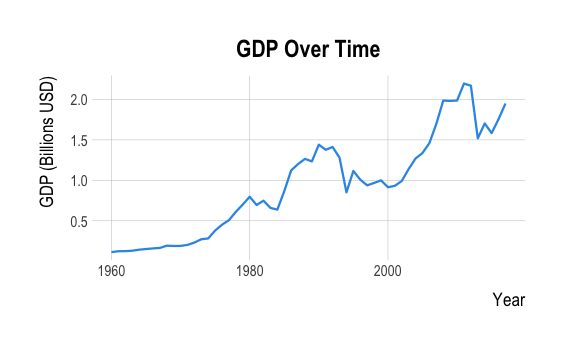
\includegraphics[width=\linewidth]{EDA/GDP_over_Time.png} % replace with your filename
    \caption{Caption for the first image.}
    \label{fig:side:a}
  \end{subfigure}
  \hfill
  %--------------- Second image ---------------
  \begin{subfigure}[b]{0.48\textwidth}
    \centering
    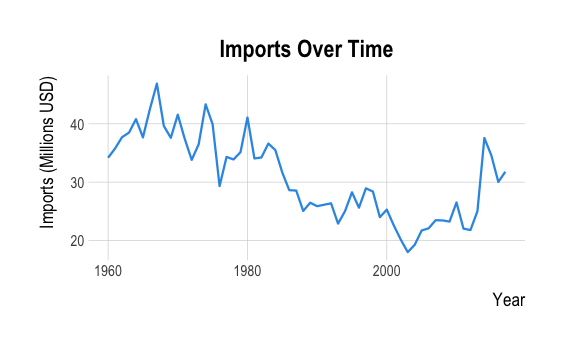
\includegraphics[width=\linewidth]{EDA/Imports_over_Time.png} % replace with your filename
    \caption{Caption for the second image.}
    \label{fig:side:b}
  \end{subfigure}

  \label{fig:side-by-side}

  \begin{subfigure}[b]{0.48\textwidth}
    \centering
    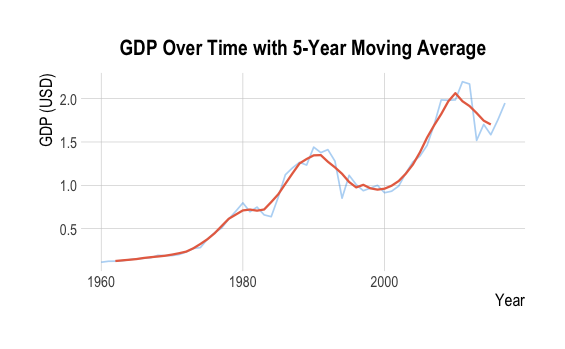
\includegraphics[width=\linewidth]{EDA/GDP_MA5.png} % replace with your filename
    \caption{Caption for the first image.}
    \label{fig:side:a}
  \end{subfigure}
  \hfill
  %--------------- Second image ---------------
  \begin{subfigure}[b]{0.48\textwidth}
    \centering
    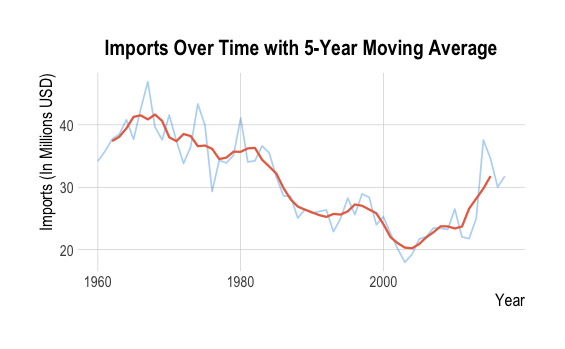
\includegraphics[width=\linewidth]{EDA/Imports_MA5.png} % replace with your filename
    \caption{Caption for the second image.}
    \label{fig:side:b}
  \end{subfigure}

  \caption{Graphs for EDA.}
\end{figure}



\end{document}

